\begin{frame}\frametitle{Theory. Proton-Proton Collisions}
%\begin{figure}[htb]
%  \begin{center}
%    {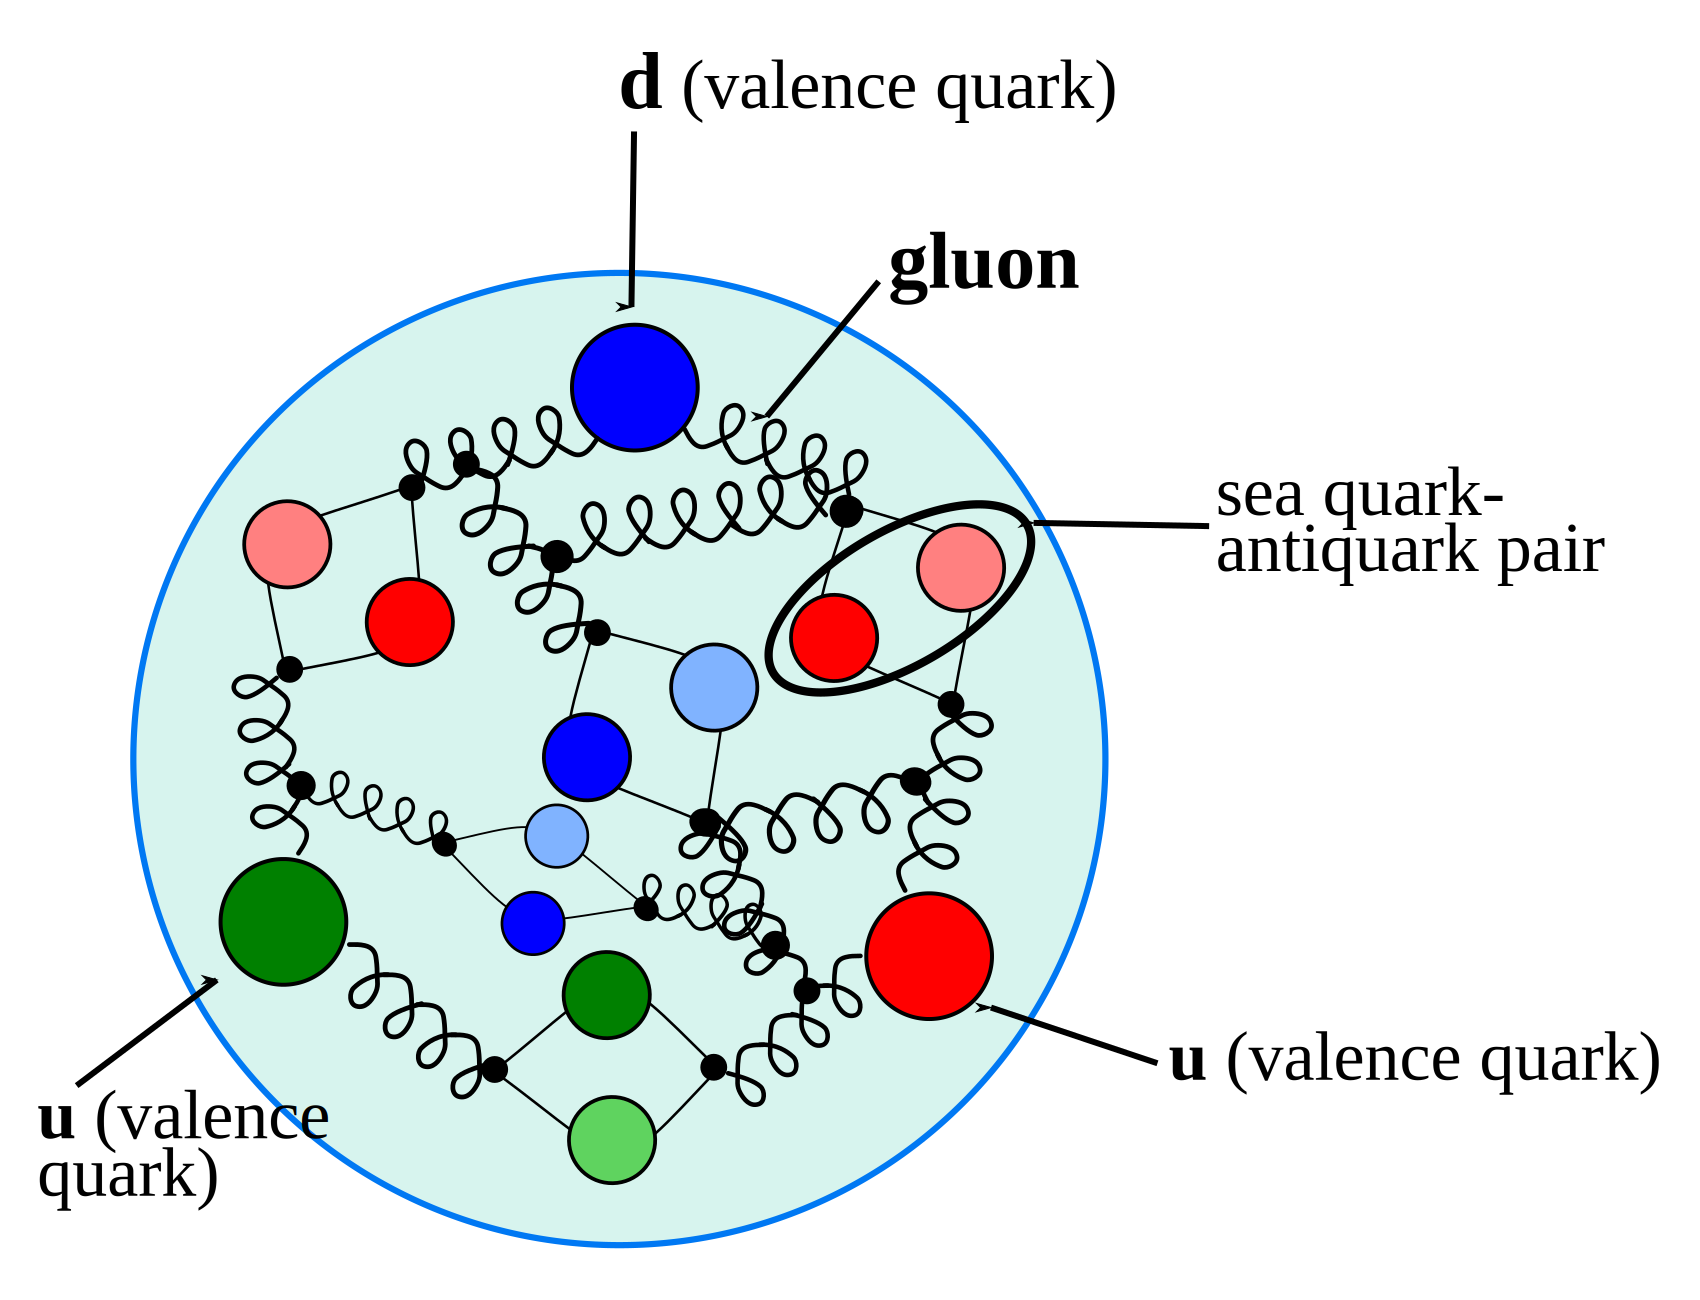
\includegraphics[width=0.45\textwidth]{../figs/Intro/protonStructure.png}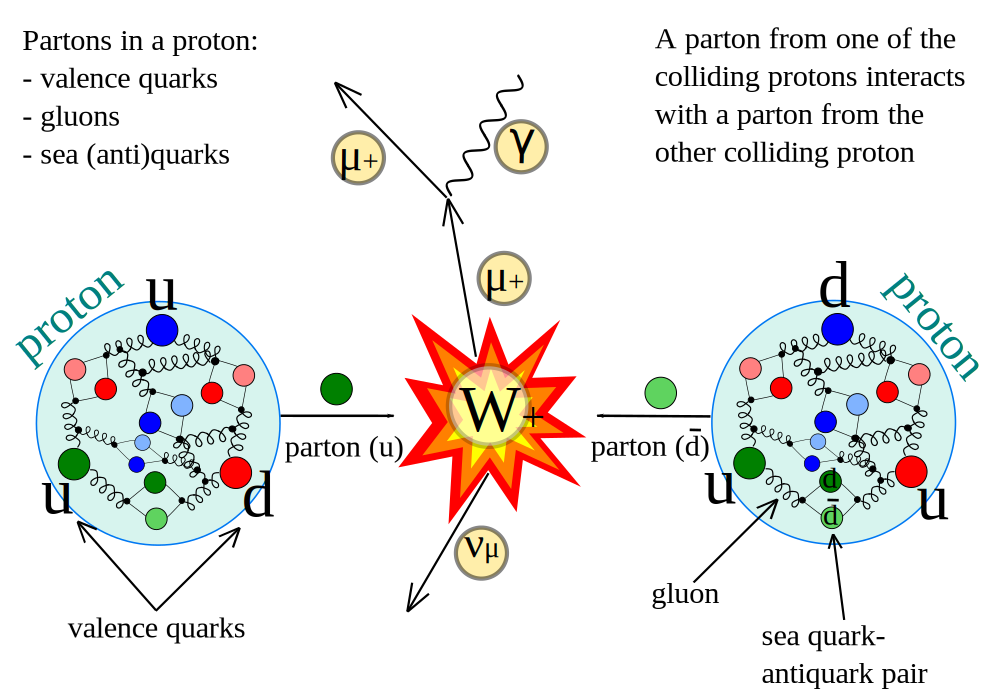
\includegraphics[width=0.45\textwidth]{../figs/Intro/ppCollision.png}}
%  \end{center}
%\end{figure}
\end{frame}%{Proton-Proton Collisions}

\begin{frame}\frametitle{Theory. EWK Interactions}

\begin{figure}[htb]
  \begin{center}
    {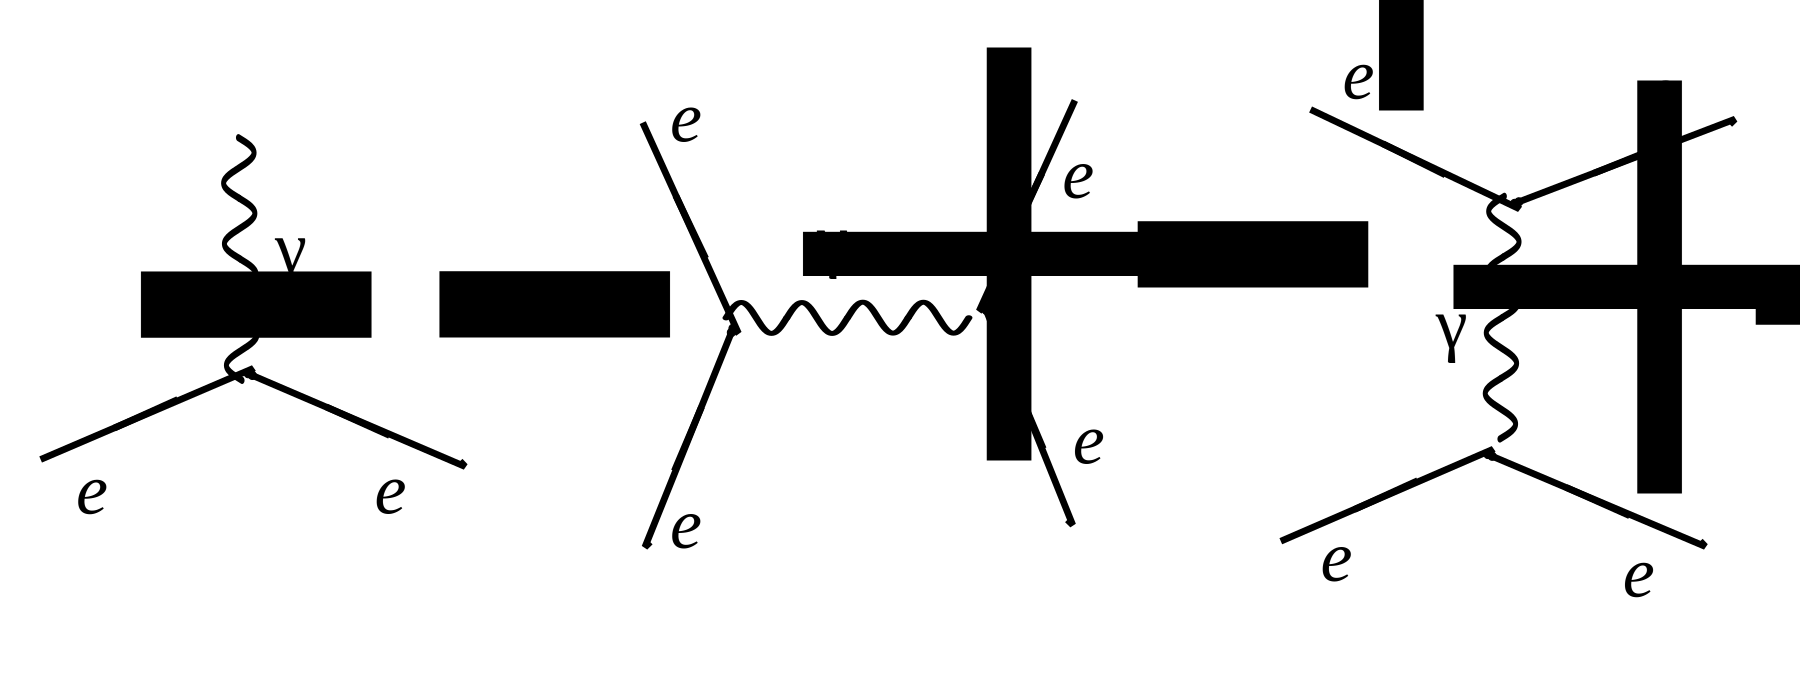
\includegraphics[width=0.50\textwidth]{../figs/Intro/feynmEM.png}}
%    \caption\tiny{Electromagnetic interactions.}
    \label{fig:feynmEM}
  \end{center}
\end{figure}

\begin{figure}[htb]
  \begin{center}
    {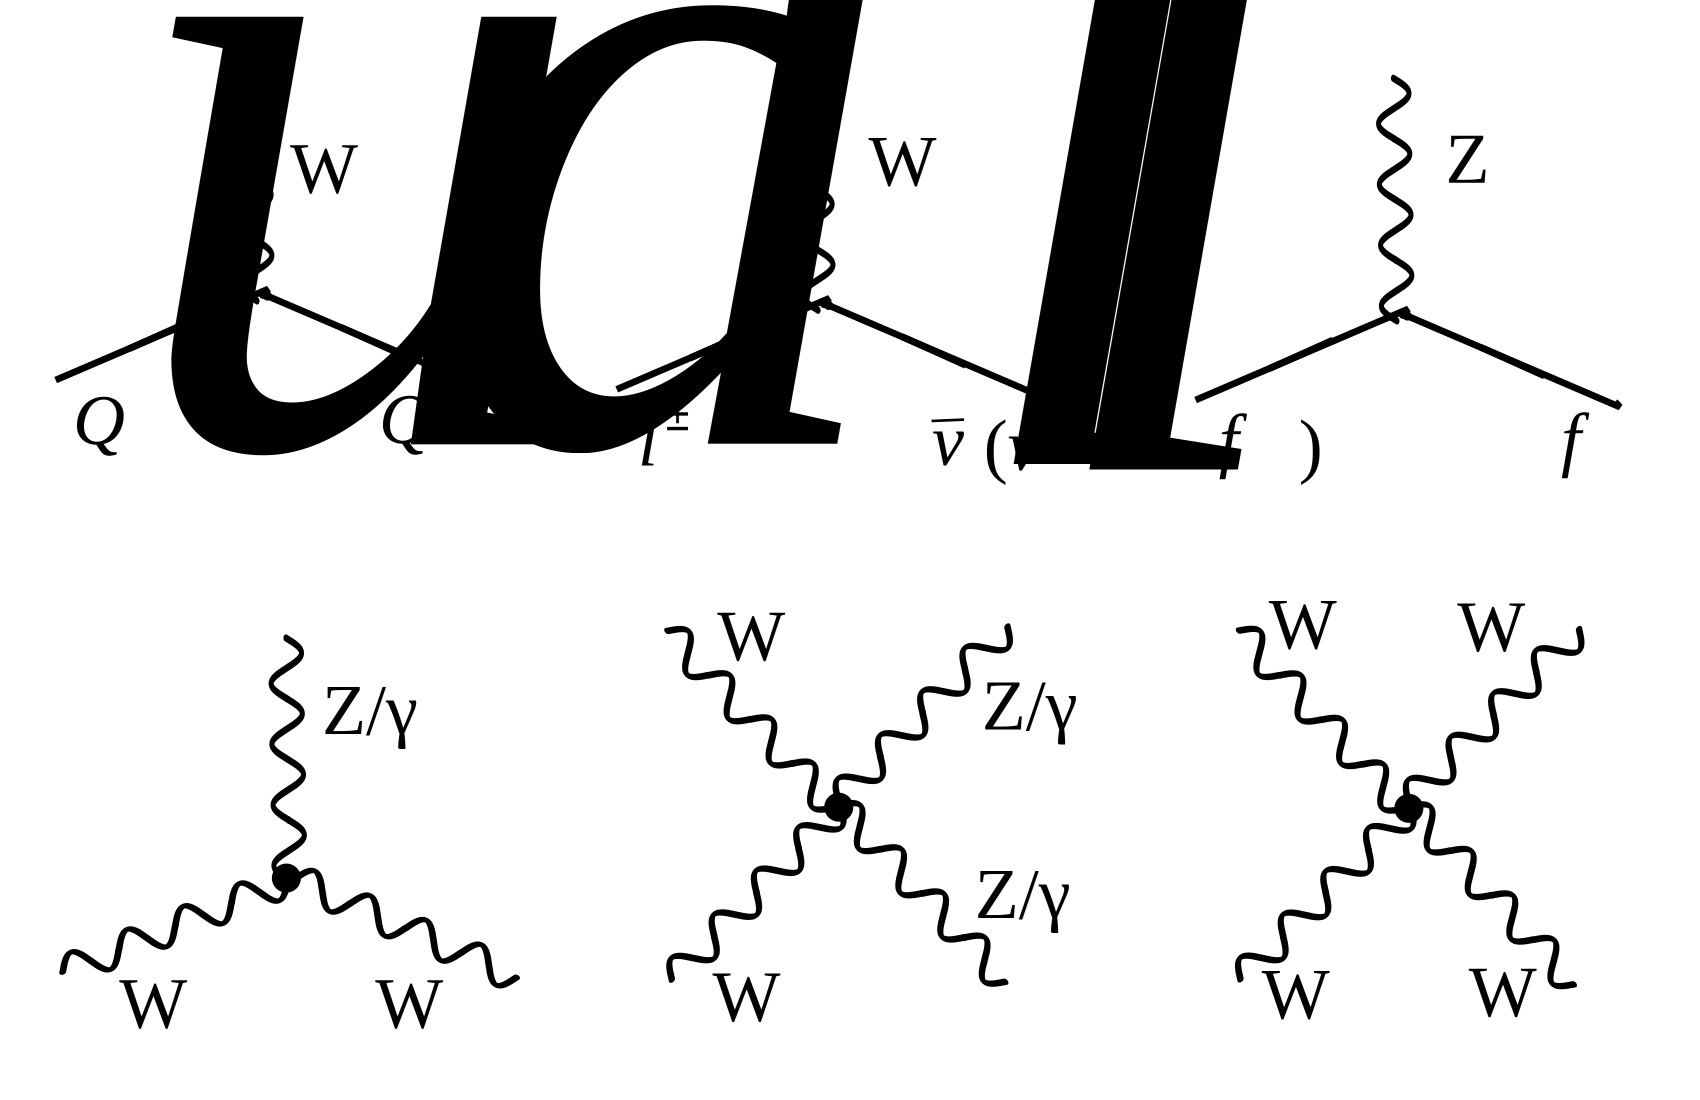
\includegraphics[width=0.50\textwidth]{../figs/Intro/feynmW.png}}
%    \caption\tiny{Weak elementary processes and gauge couplings.}
    \label{fig:feynmW}
  \end{center}
\end{figure}

  \scriptsize
   W decay channels:

\end{frame}%{Theory. Weak Interactions}

%\begin{frame}\frametitle{Theory. Anomalous Gauge Couplings}
%\begin{figure}[htb]
%  \begin{center}
%    {\includegraphics[width=0.95\textwidth]{../figs/WgAbout/TGC_and_QGC_vertices.png}}
%    \caption\tiny{Charged TGC (first), neutral TGC (second), charged QGC (third and fourth), and neutral QGC (fifth) vertices.}
%    \label{fig:TGC_and_QGC_vertices}
%  \end{center}
%\end{figure}
%\end{frame}%{Theory. Anomalous Gauge Couplings}

\begin{frame}\frametitle{Theory. $W\gamma\rightarrow l\nu\gamma$}

   \begin{figure}[htb]
      \begin{center}
        \scriptsize
          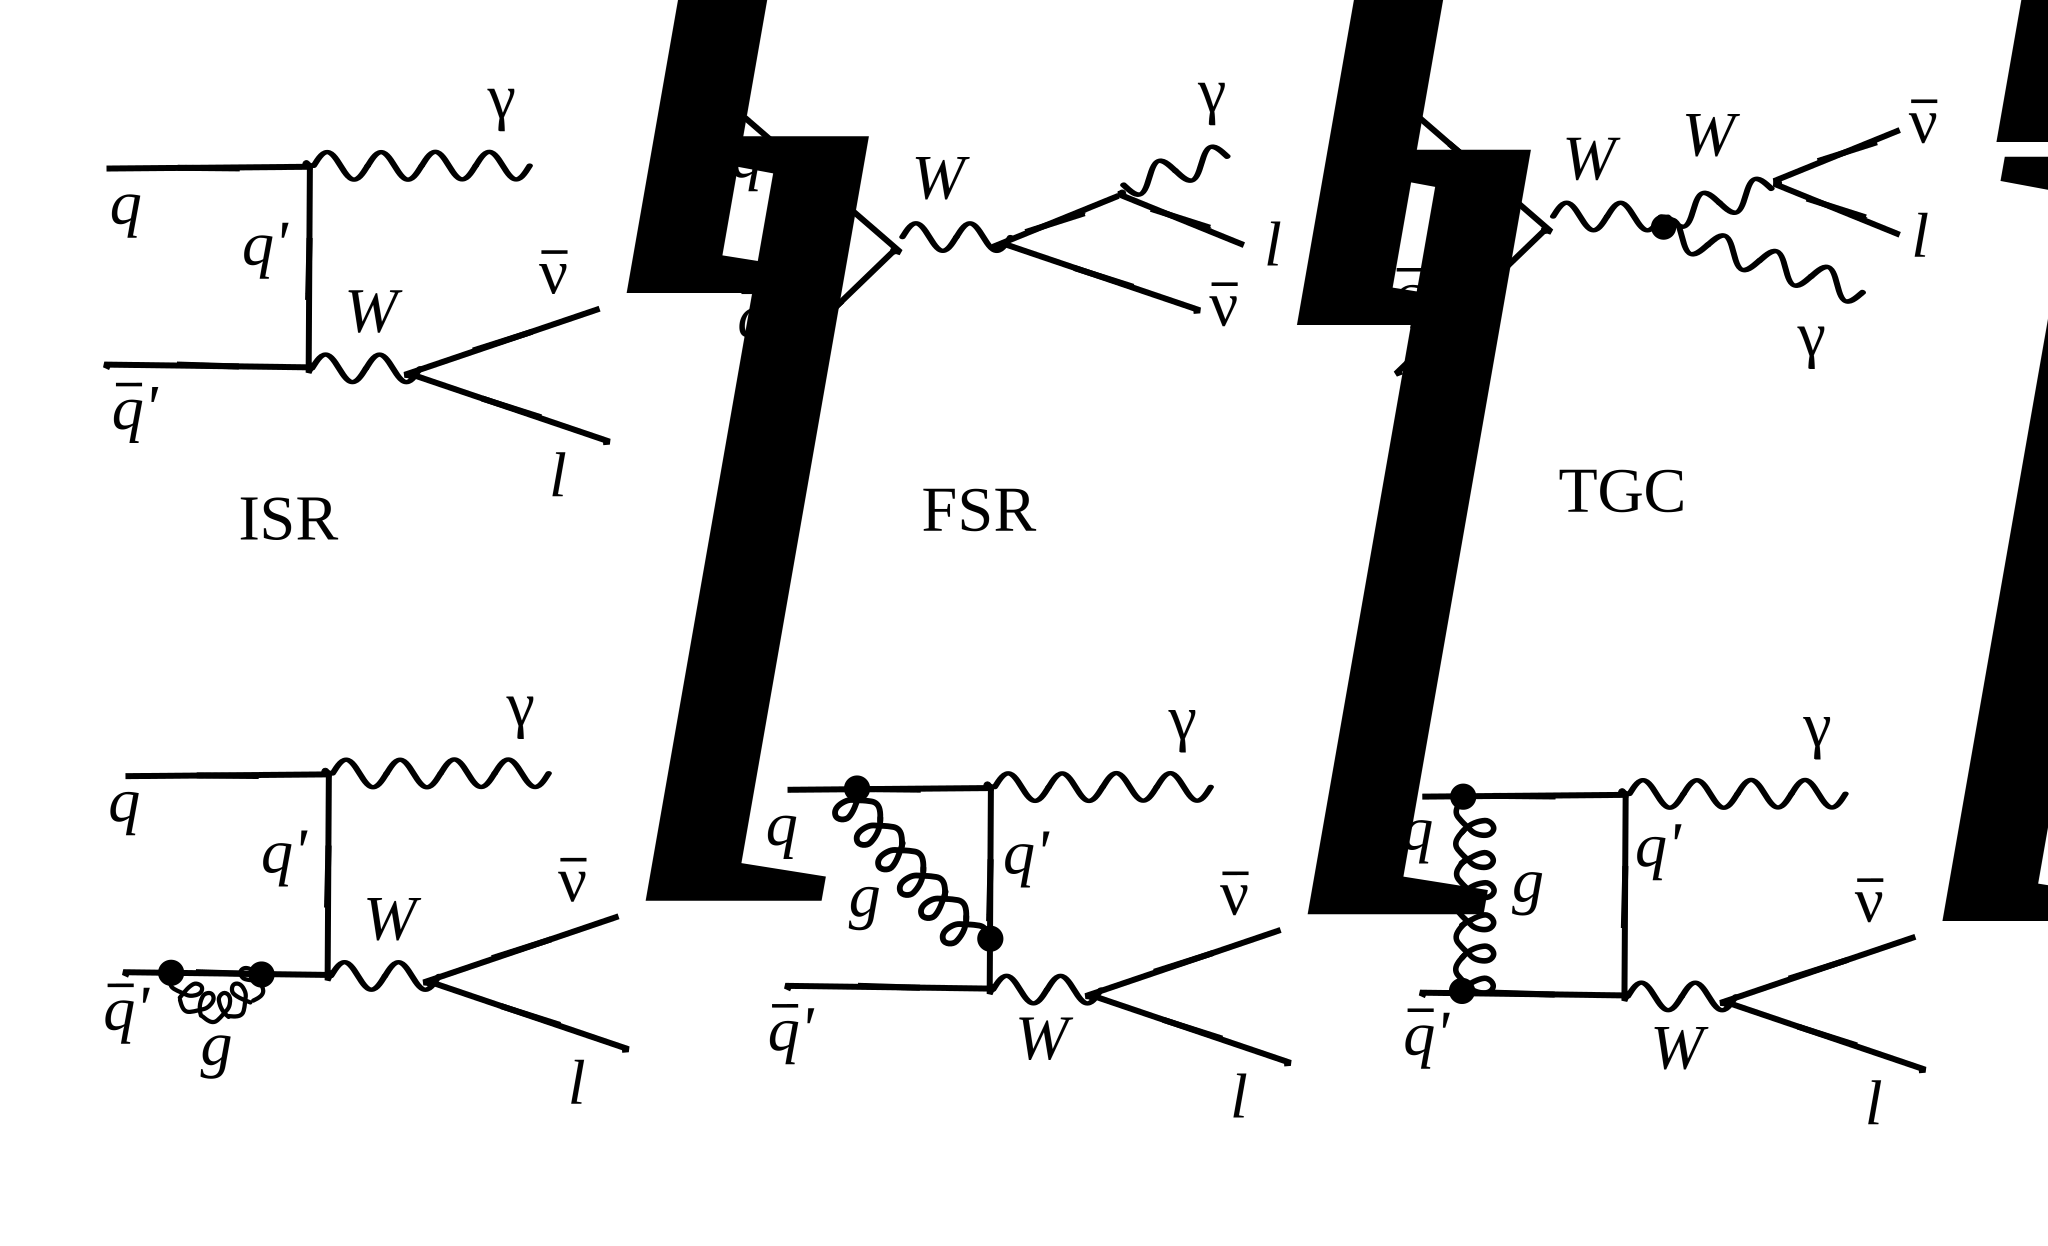
\includegraphics[width=0.95\textwidth]{../figs/WgAbout/feynmWg_LO_NLO.png}
%          \caption{\scriptsize{The Feynman diagrams. ISR(x2), FSR, and TGC.}}
       \end{center}
    \end{figure}

  \begin{itemize}
    \scriptsize
    \item test Standard Model;
    \item search for aTGC.
  \end{itemize}
\end{frame}%{Theory. $W\gamma\rightarrow l\nu\gamma$}
